\section{Experiments}
\label{sec:experiment}

We evaluate MgfrOFR under two complementary settings. Synthetic clips include ground truth and therefore support full-reference fidelity and perceptual metrics. Real archival footage lacks ground truth, so only no-reference naturalness metrics apply. We keep these settings separate throughout this section because a single merged score would mask the fidelity--naturalness trade-off that defines old film restoration.

\subsection{Datasets and Evaluation Metrics}
\label{subsec:datasets_metrics}

\subsubsection{Datasets}
\label{subsec:datasets}

We evaluate MgfrOFR on the SRWOV benchmark introduced with MambaOFR~\cite{mao2025mambaofr}, a dedicated old film restoration benchmark that provides both synthetic and real-world test sets.

For training, we use the REDS training split~\cite{nah2019reds}, which contains 240 video sequences, each with 100 frames at $720 \times 1280$ resolution. Clean REDS frames are degraded on the fly with the synthetic degradation pipeline from MambaOFR, which simulates scratches, dust, blotches, flicker, and grain and produces paired degraded and clean training samples.

The synthetic test set contains 30 clips rendered with the same degradation pipeline on held-out REDS sequences. Each clip has 100 frames at $720 \times 1280$ with paired ground truth, enabling full-reference scoring. The real-world set contains 216 clips of archival footage from the 1920s to the 1960s, with authentic mixed degradations and no ground truth. We follow the original 216-clip SRWOV protocol~\cite{mao2025mambaofr}. It spans indoor portraits, newsreel footage, conversations, and multi-person scenes, and totals 29{,}256 frames for a broad naturalness assessment.

\subsubsection{Evaluation Metrics}
\label{subsec:eval_metrics}

Seven metrics cover three complementary dimensions. On synthetic data with ground truth, we report PSNR and SSIM~\cite{wang2004ssim} for pixel fidelity (higher is better), LPIPS~\cite{zhang2018lpips} for learned perceptual distance (lower is better), and DISTS~\cite{ding2020dists} for joint structure-texture similarity (lower is better). On real data without ground truth, we use NIQE~\cite{mittal2012niqe} and BRISQUE~\cite{mittal2012brisque} for statistical naturalness (lower is better), together with CLIP-IQA+~\cite{wang2023clipiqa}, which evaluates CLIP~\cite{radford2021clip} features through learnable quality-aware prompts (higher is better). These groups probe pixel fidelity, perceptual quality, and naturalness in turn.

\subsection{Implementation Details}
\label{subsec:implementation}

\subsubsection{Training Details}
\label{subsubsec:training_details}

We train MgfrOFR on the REDS training split~\cite{nah2019reds} with the synthetic degradation pipeline from Section~\ref{subsec:datasets}. The optimizer is Adam~\cite{kingma2015adam} with $\beta_1=0.9$ and $\beta_2=0.99$, an initial learning rate of $2\times10^{-4}$, and a MultiStep schedule with milestones at 50K, 100K, and 150K iterations ($\gamma=0.5$). Training runs for $200$K iterations on $4$ NVIDIA A100 GPUs (80\,GB each), one clip per GPU per mini-batch. Each sample is $T=7$ consecutive frames cropped to $256\times256$. We use PyTorch 2.7 with CUDA 12.4 and fix the random seed to 42. At inference, RATR is off and frames are processed at full $720 \times 1280$ resolution without cropping.

\subsubsection{Baseline Adaptation Protocol}
\label{subsubsec:baseline_adaptation}

The comparison reuses released implementations and published settings in one unified environment. For clarity, we make each baseline's adaptation explicit along four axes.

\textbf{Retraining and computational budget.} Dedicated old film restoration methods (RTN, RRTN, MambaOFR) are retrained under the same REDS-based synthetic film degradation pipeline as MgfrOFR. In particular, MambaOFR---our primary baseline---and MgfrOFR are trained with an identical 200K-iteration schedule on the same A100-class hardware, so their computational budget for old film restoration adaptation is matched; RTN and RRTN are reproduced under the same degradation pipeline with a comparable training budget.

\textbf{Hyper-parameter tuning.} We retain each baseline's published architecture-specific hyper-parameters rather than performing exhaustive per-baseline re-tuning. Re-tuning every method to convergence on old film restoration would be computationally prohibitive and could bias the comparison toward whichever baseline received the most tuning effort.

\textbf{Degradation adaptation.} Generic video restoration methods (VRT, RVRT, ShiftNet) keep their published architecture and default optimization recipe; we replace only the task-specific degradation generation so that they can be trained on old film restoration inputs, and we report them as faithfully reproduced references whose training budget follows each released recipe.

\textbf{Reference systems.} Enhancement-oriented methods (DeOldify, OldPhoto, DeepRemaster) are not designed for paired old film restoration and are not retrained on the old film restoration pipeline; we include them strictly as reference systems to contextualize perceptual trade-offs, not as task-matched old film restoration baselines.

The comparison is therefore a unified reproduction study under a shared degradation protocol, with a budget-matched tier for dedicated old film restoration methods. It does not claim that every baseline has been exhaustively re-optimized for old film restoration.

\subsection{Comparison with State-of-the-Art}
\label{subsec:comparison_sota}

We compare MgfrOFR against nine baselines spanning dedicated old film restoration methods, general video restoration models, and image/video enhancement approaches. The dedicated old film restoration baselines are RTN~\cite{wan2022rtn}, RRTN~\cite{lin2024rrtn}, and MambaOFR~\cite{mao2025mambaofr}; the general video restoration baselines are VRT~\cite{liang2024vrt}, RVRT~\cite{liang2022rvrt}, and ShiftNet~\cite{li2023shiftnet}; and the enhancement-oriented references are DeOldify~\cite{jantic2019deoldify}, OldPhoto~\cite{wan2023oldphotopami}, and DeepRemaster~\cite{iizuka2019deepremaster}. No-reference metrics are computed using the pyiqa library under the same software environment.

\subsubsection{Quantitative Comparison on Synthetic Data}

On the SRWOV synthetic benchmark with full-reference metrics (Table~\ref{tab:sota}), MgfrOFR ranks first on all four reported metrics. It reaches 27.86~dB PSNR and improves on the same-protocol MambaOFR baseline by +1.02~dB with the final average-fusion configuration. The ranking is consistent with the architectural gap between method families: generic video restoration models include no defect handling specific to old film restoration, while frame-wise enhancement methods can break temporal consistency.

\begin{table}[htbp]
\caption{Quantitative comparison of SRWOV synthetic full-reference results under the unified reproduction protocol. Best results are shown in \bestres{red} and second-best results in \secondres{blue}.\label{tab:sota}}
\begin{tabularx}{\textwidth}{lCCCC}
\toprule
\textbf{Method} & \textbf{PSNR$\uparrow$} & \textbf{SSIM$\uparrow$} & \textbf{LPIPS$\downarrow$} & \textbf{DISTS$\downarrow$} \\
\midrule
ShiftNet~\cite{li2023shiftnet}          & 21.48 & 0.8234 & 0.2030 & 0.1303 \\
VRT~\cite{liang2024vrt}                 & 22.39 & 0.8631 & 0.1750 & 0.1087 \\
RVRT~\cite{liang2022rvrt}              & 22.43 & 0.8710 & 0.1655 & 0.1078 \\
DeOldify~\cite{jantic2019deoldify}      & 23.22 & 0.8923 & 0.2775 & 0.1260 \\
RRTN~\cite{lin2024rrtn}                & 24.15 & 0.9006 & 0.1082 & \secondres{0.0668} \\
OldPhoto~\cite{wan2023oldphotopami}     & 24.62 & 0.8524 & 0.2252 & 0.1144 \\
DeepRemaster~\cite{iizuka2019deepremaster} & 25.06 & \secondres{0.9185} & 0.1108 & 0.0895 \\
RTN~\cite{wan2022rtn}                   & 25.85 & 0.8869 & 0.1214 & 0.0862 \\
MambaOFR~\cite{mao2025mambaofr}        & \secondres{26.84} & 0.9153 & \secondres{0.0719} & 0.0733 \\
\midrule
MgfrOFR (Ours)                          & \bestres{27.86} & \bestres{0.9255} & \bestres{0.0600} & \bestres{0.0656} \\
\bottomrule
\end{tabularx}
\end{table}

A single average score can hide clip-level variance, so we include the paired, two-sided Wilcoxon signed-rank test over the 30 per-clip means as supporting evidence. For the final average-fusion configuration, MgfrOFR obtains significant paired improvements over MambaOFR on all four full-reference metrics (PSNR $p=3.73\times10^{-9}$; SSIM $p=1.73\times10^{-6}$; LPIPS $p=1.86\times10^{-9}$; DISTS $p=1.92\times10^{-6}$). Per-clip evidence further shows that PSNR and DISTS improve on 29 of 30 clips, while SSIM and LPIPS improve on all 30 clips.

\subsubsection{Quantitative Comparison on Real-World Data}

Table~\ref{tab:realworld} reports no-reference quality on the 216 real-world clips. No real-world clip has a reference, and all methods are evaluated in the same pyiqa-based metric environment on the full 216-clip set. NIQE and BRISQUE measure statistical naturalness, while CLIP-IQA+ reflects CLIP-aligned perceptual quality; because they capture different attributes, we report each one individually instead of merging them into a single score.

\begin{table}[htbp]
\caption{Real-world evaluation of no-reference quality metrics on SRWOV real footage under the same pyiqa-based metric environment. Best results are shown in \bestres{red} and second-best results in \secondres{blue}.\label{tab:realworld}}
\begin{tabularx}{\textwidth}{lCCC}
\toprule
\textbf{Method} & \textbf{NIQE$\downarrow$} & \textbf{BRISQUE$\downarrow$} & \textbf{CLIP-IQA+$\uparrow$} \\
\midrule
ShiftNet~\cite{li2023shiftnet}             & 5.71  & 42.82 & 0.3975 \\
VRT~\cite{liang2024vrt}                    & 5.66  & 42.73 & 0.3985 \\
RVRT~\cite{liang2022rvrt}                 & 5.72  & 42.64 & 0.4013 \\
DeOldify~\cite{jantic2019deoldify}         & 5.72  & 41.61 & 0.3768 \\
RRTN~\cite{lin2024rrtn}                   & 5.67  & 32.86 & 0.3969 \\
OldPhoto~\cite{wan2023oldphotopami}        & 6.56  & 30.45 & \bestres{0.4503} \\
DeepRemaster~\cite{iizuka2019deepremaster} & 5.99  & 40.62 & 0.3991 \\
RTN~\cite{wan2022rtn}                      & \secondres{5.17}  & \bestres{19.00} & 0.4163 \\
MambaOFR~\cite{mao2025mambaofr}           & 5.34  & 29.79 & \secondres{0.4351} \\
\midrule
MgfrOFR (Ours)                             & \bestres{5.12}  & \secondres{24.79} & 0.4092 \\
\bottomrule
\end{tabularx}
\end{table}

MgfrOFR obtains the best NIQE (5.12) and the second-best BRISQUE (24.79) among all compared methods, improving over MambaOFR on both NIQE (5.12 vs.\ 5.34) and BRISQUE (24.79 vs.\ 29.79). Its CLIP-IQA+ (0.4092) remains below OldPhoto (0.4503), MambaOFR (0.4351), and RTN (0.4163). This gap is consistent with CLIP-IQA+'s tendency to favor sharper, enhancement-oriented outputs, whereas our granularity recalibration remains conservative and favors statistical naturalness. We analyze this naturalness-versus-enhancement trade-off in Section~\ref{subsec:failure}.

\subsubsection{Qualitative Comparison}

Figure~\ref{fig:qualitative_synthetic} compares four representative REDS-synthetic scenes using full-frame degraded inputs and enlarged ROI crops. The colored boxes in the input row mark local regions, and subsequent rows compare the corresponding crops across restoration methods and the ground truth. The method families fail in different ways. General video restoration removes part of the photometric degradation but leaves structured defects largely intact. Enhancement baselines raise contrast, yet blur or hallucinate local texture. RTN and MambaOFR clear many visible defects but still lose fine structure inside damaged regions. MgfrOFR stays closest to the ground-truth edges and textures around scratches, blotches, and high-contrast damage while suppressing residual old-film artifacts. This behavior is consistent with the PSNR advantage in Table~\ref{tab:sota}. Supplementary Video~S1 provides side-by-side temporal comparisons in two parts: a synthetic part against the ground truth on REDS-synthetic clips with per-frame PSNR, followed by a real-world part on SRWOV archival clips annotated with the overall no-reference NIQE and BRISQUE.

\begin{figure}[!htbp]
\begin{adjustwidth}{-\extralength}{0cm}
\centering
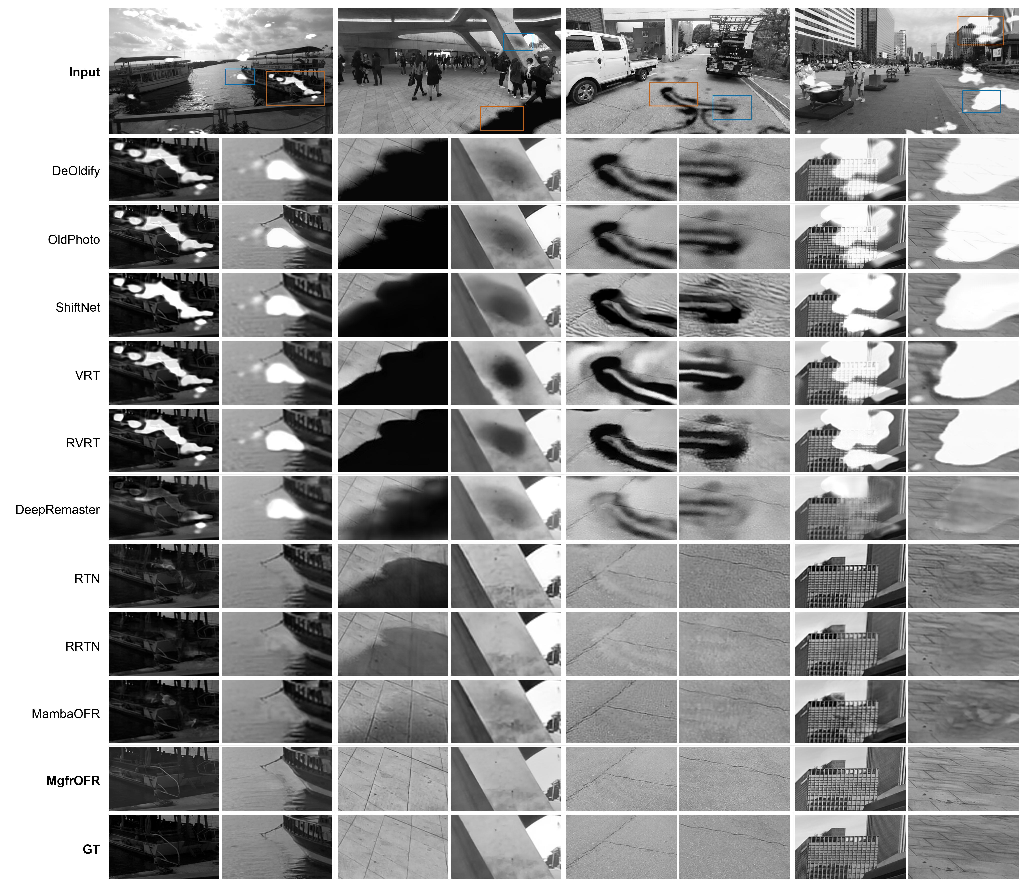
\includegraphics[width=1.31\textwidth]{figures/Fig4_SOTA_Synthetic_REDS_synthetic_Qualitative.pdf}
\end{adjustwidth}
\caption{Qualitative comparison on four representative REDS-synthetic scenes. The top row shows full degraded input frames with colored ROI boxes, and the following rows compare enlarged ROI crops from DeOldify, OldPhoto, ShiftNet, VRT, RVRT, DeepRemaster, RTN, RRTN, MambaOFR, MgfrOFR (Ours), and the ground truth. The comparison shows that MgfrOFR better preserves local edges and texture details around scratches while reducing visible old-film artifacts across the selected scenes.\label{fig:qualitative_synthetic}}
\end{figure}

Figure~\ref{fig:qualitative_realworld} compares three representative RealFilm-SRWOV real-world clips covering facial close-ups, indoor scenes, and high-contrast local structures. Because no ground truth is available, the comparison focuses on visible artifact suppression, structural preservation, naturalness, and local texture in the enlarged ROI crops. General video restoration clears part of the photometric degradation but leaves residual scratches, stains, or contrast shifts. Enhancement baselines sharpen texture, yet can over-enhance faces, clothing, and high-contrast boundaries. MgfrOFR maintains facial structure, fabric texture, object boundaries, and local contrast more consistently than MambaOFR and the other old film restoration baselines, while suppressing residual old-film artifacts. These observations are consistent with the best NIQE and the BRISQUE improvement over MambaOFR in Table~\ref{tab:realworld}, while CLIP-IQA+ reflects a separate sharpness-oriented trade-off. Two failure modes remain: MgfrOFR can over-smooth very fine texture under extreme degradation, and severe motion blur still causes flow-alignment errors, both examined in Section~\ref{subsec:failure}.

\begin{figure}[!htbp]
\begin{adjustwidth}{-\extralength}{0cm}
\centering
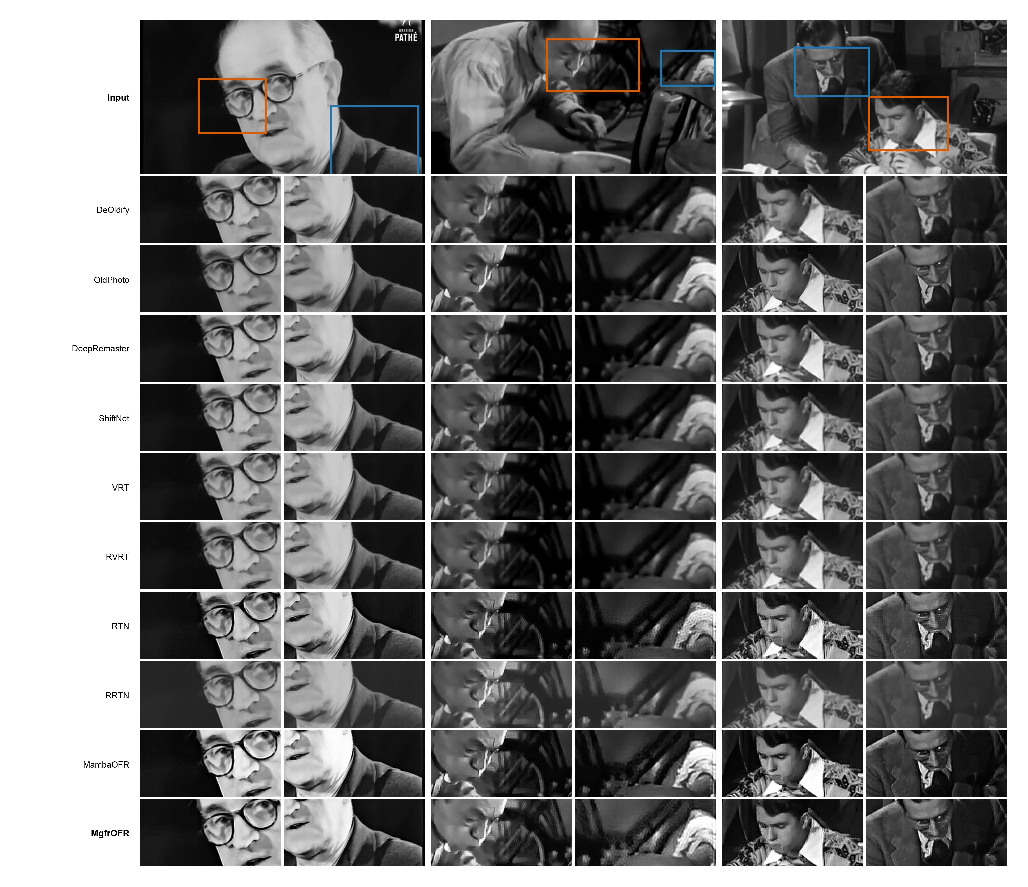
\includegraphics[width=1.31\textwidth]{figures/Fig5_SOTA_RealWorld_RealFilm_SRWOV_Qualitative.pdf}
\end{adjustwidth}
\caption{Qualitative comparison on three representative RealFilm-SRWOV real-world clips. The input row shows degraded frames with colored ROI boxes, and the following rows compare enlarged ROI crops from DeOldify, OldPhoto, DeepRemaster, ShiftNet, VRT, RVRT, RTN, RRTN, MambaOFR, and MgfrOFR (Ours). Because these clips have no ground truth, the crops compare visible local restoration details across methods. The comparison shows that MgfrOFR suppresses residual old-film artifacts while preserving natural structure and local texture without relying on ground-truth references.\label{fig:qualitative_realworld}}
\end{figure}

\FloatBarrier

\subsection{Ablation Study}
\label{subsec:ablation}

Table~\ref{tab:ablation} isolates the two contributions, MGFE recalibration and RATR regularization. These ablation values are used only for module analysis and do not replace the main comparison in Table~\ref{tab:sota}. Setting names match Figure~\ref{fig:ablation_visual}. The +RATR-only row is a partial control: MGFE branch descriptors still serve as RATR ranking targets, but channel-wise recalibration is switched off.

\begin{table}[htbp]
\scriptsize
\caption{Ablation study on the SRWOV synthetic benchmark. The setting names follow Figure~\ref{fig:ablation_visual}, with max fusion retained as a tabular control; ``MGFE'' denotes channel-wise recalibration in this table. Best results are shown in \bestres{red} and second-best results in \secondres{blue}.\label{tab:ablation}}
\centering
\begin{adjustwidth}{-\extralength}{0cm}
\begingroup
\renewcommand{\arraystretch}{1.04}
\begin{tabularx}{\fulllength}{l*{6}{>{\centering\arraybackslash}X}}
\toprule
\textbf{Setting} & \textbf{MGFE} & \textbf{RATR} & \textbf{PSNR$\uparrow$} & \textbf{SSIM$\uparrow$} & \textbf{LPIPS$\downarrow$} & \textbf{DISTS$\downarrow$} \\
\midrule
MambaOFR baseline               & Off & Off & 26.84 & 0.9153 & 0.0719 & 0.0733 \\
+MGFE only                      & On  & Off & \secondres{27.75} & 0.9219 & 0.0651 & 0.0702 \\
+RATR only                      & Off & On  & 27.72 & \secondres{0.9246} & \secondres{0.0646} & \secondres{0.0696} \\
MgfrOFR (max-fusion control)   & On  & On  & 27.17 & 0.9168 & 0.0740 & 0.0773 \\
MgfrOFR (average fusion)       & On  & On  & \bestres{27.86} & \bestres{0.9255} & \bestres{0.0600} & \bestres{0.0656} \\
\bottomrule
\end{tabularx}
\endgroup
\end{adjustwidth}
\end{table}

\FloatBarrier

\noindent\textbf{Discussion.} Within this ablation protocol, the full model achieves the best values for all four metrics and improves the MambaOFR baseline by +1.02~dB PSNR. Each component helps on its own, but neither is sufficient. MGFE-only recalibration lifts the baseline yet trails the full model on LPIPS and DISTS, so recalibration alone does not deliver the best fidelity--perception balance. RATR-only regularization gives a similar PSNR gain with a better perceptual balance than MGFE-only recalibration, showing that ranking diversity is beneficial even before channel-wise feedback is enabled. Average fusion combines the two into the strongest result. The max-fusion control shows negative synergy on all four full-reference metrics and justifies average fusion as the default.

\begin{figure}[htbp]
\centering
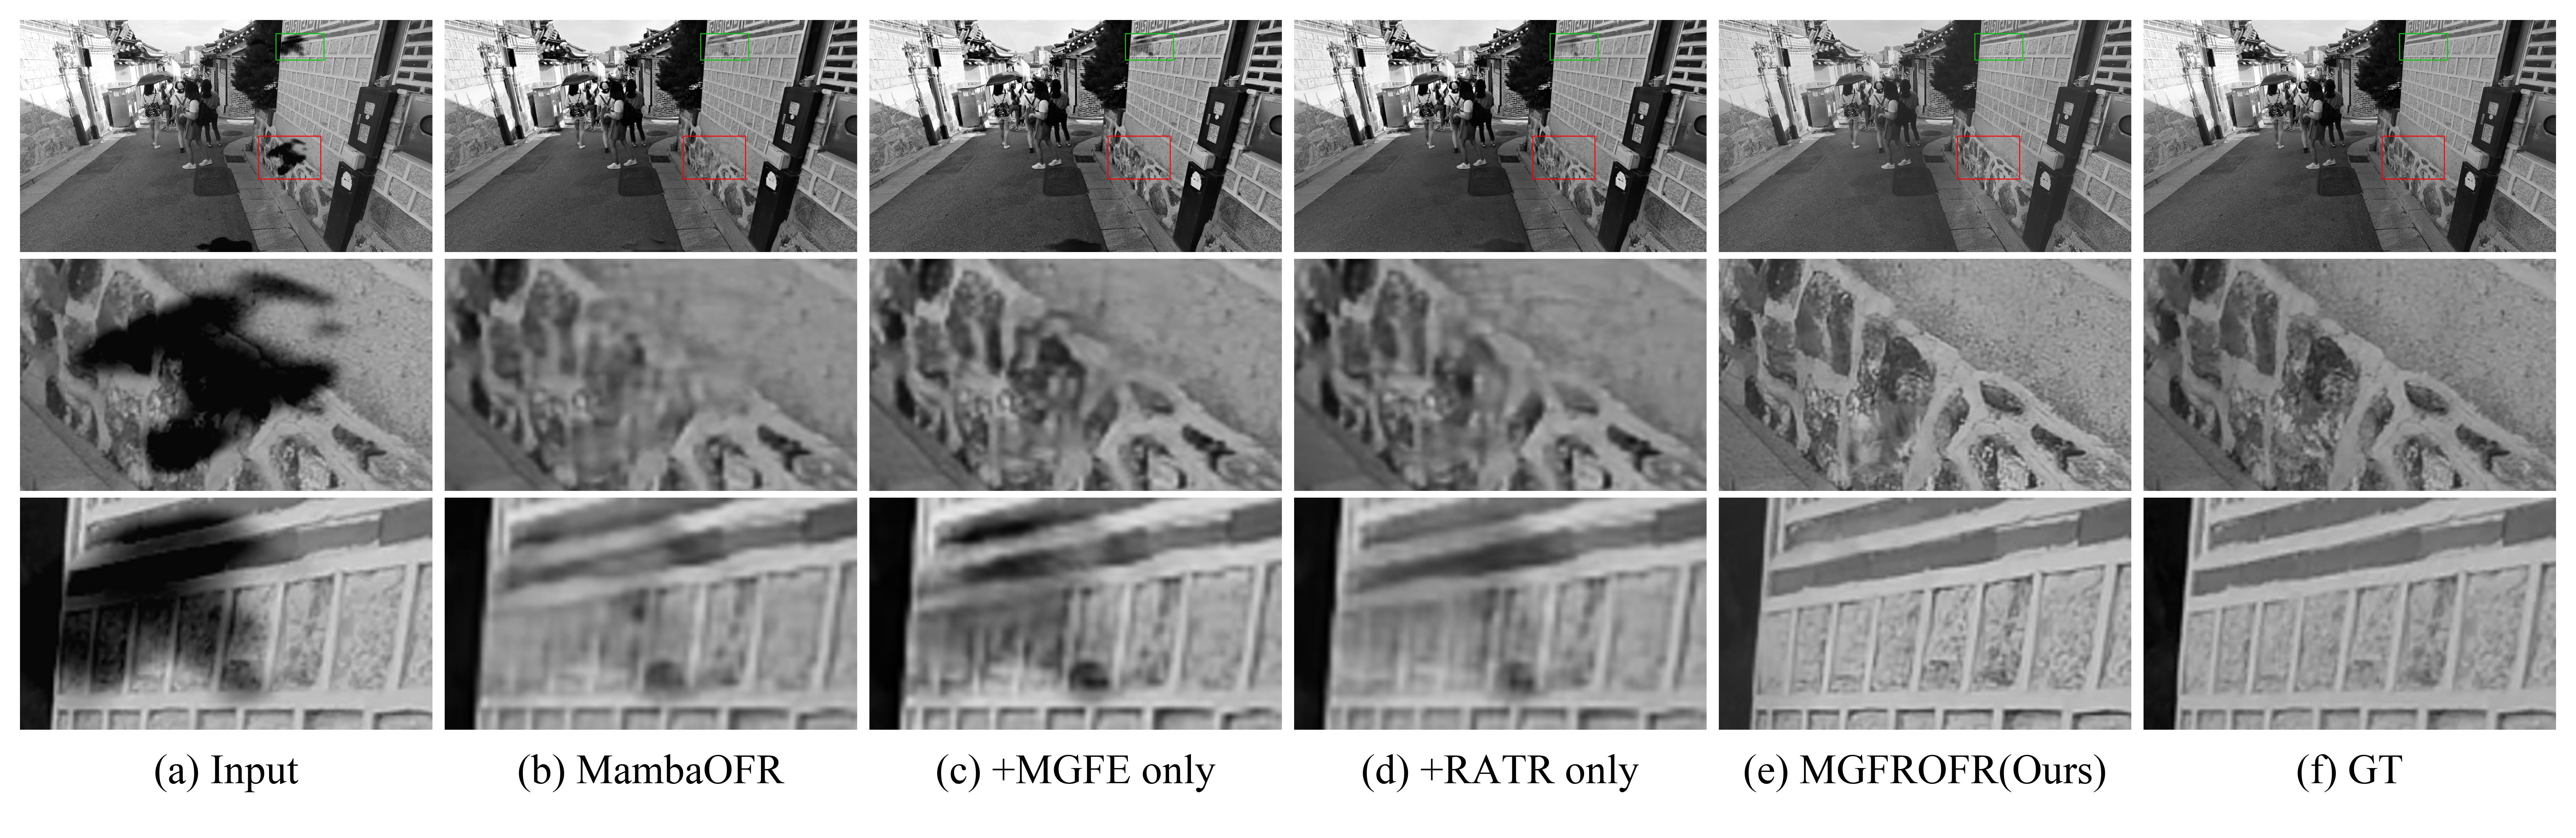
\includegraphics[width=0.95\textwidth]{figures/Fig6_Ablation_REDS_synthetic_Qualitative.jpg}
\caption{Visual ablation on REDS-based SRWOV synthetic data. \textbf{Top row:} full frames with red and green crop boxes marking the zoom regions. \textbf{Middle and bottom rows:} zoomed patches from the marked regions. The restoration columns compare the MambaOFR baseline, +MGFE only, +RATR only, and MgfrOFR with average fusion, with the degraded input and ground truth included as references. The max-fusion control is omitted for visual clarity. The comparison shows that combining MGFE with RATR under average fusion yields the cleanest local restoration among the ablated configurations in Table~\ref{tab:ablation}.\label{fig:ablation_visual}}
\end{figure}

\subsection{Hyperparameter Sensitivity}
\label{subsec:sensitivity}

We report sensitivity and design-control entries only for configurations with complete evaluation records under the stated protocol. The main MgfrOFR configuration uses average restoration-token fusion, while the earlier max-fusion configuration is retained as a fusion control. Table~\ref{tab:sensitivity_granularity} covers granularity controls, a lower-temperature ranking control, token-insertion control, and branch-aggregation control. The token-insertion and branch-aggregation settings are treated as predefined max-fusion controls rather than alternatives to the average-fusion main configuration.

\begin{table}[H]
\caption{Sensitivity and design-control results on REDS synthetic data. The table combines a granularity sweep and fixed-size controls under the stated evaluation protocol; $M$ denotes the number of restoration tokens and $G$ denotes the number of granularity branches. MgfrOFR denotes the average-fusion main configuration, while the control rows are retained only for diagnostic comparison. Best results are shown in \bestres{red} and second-best results in \secondres{blue}.\label{tab:sensitivity_granularity}}
\centering
\begin{adjustwidth}{-\extralength}{0cm}
\begingroup
\scriptsize
\setlength{\tabcolsep}{3.5pt}
\renewcommand{\arraystretch}{1.04}
\begin{tabularx}{\fulllength}{@{}>{\hsize=1.60\hsize\raggedright\arraybackslash}Xcc*{4}{>{\hsize=0.85\hsize\centering\arraybackslash}X}@{}}
\toprule
\textbf{Configuration} & \textbf{Tokens} & \textbf{Branches} & \textbf{PSNR$\uparrow$} & \textbf{SSIM$\uparrow$} & \textbf{LPIPS$\downarrow$} & \textbf{DISTS$\downarrow$} \\
\midrule
\multicolumn{7}{@{}l}{\textit{Granularity sweep}} \\
$G{=}1$, $M{=}4$                      & 4  & 1 & \bestres{27.95} & \bestres{0.9263} & 0.2153 & 0.1554 \\
$G{=}2$, $M{=}8$                      & 8  & 2 & 27.49 & 0.9211 & 0.2162 & 0.1557 \\
MgfrOFR (average fusion; $G{=}3$, $M{=}12$) & 12 & 3 & \secondres{27.86} & \secondres{0.9255} & \bestres{0.0600} & \bestres{0.0656} \\
$G{=}4$, $M{=}16$                     & 16 & 4 & 27.53 & 0.9197 & 0.2169 & 0.1565 \\
\addlinespace[1pt]
\midrule
\multicolumn{7}{@{}l}{\textit{Fixed 12-token / 3-branch controls}} \\
Lower ranking temperature ($\tau{=}0.05$) & 12 & 3 & 26.87 & 0.9177 & 0.0672 & 0.0717 \\
Prepend token insertion               & 12 & 3 & 27.61 & 0.9234 & \secondres{0.0627} & \secondres{0.0694} \\
Max branch aggregation                & 12 & 3 & 27.55 & 0.9223 & 0.0679 & 0.0730 \\
\bottomrule
\end{tabularx}
\endgroup
\end{adjustwidth}
\end{table}

The granularity controls reveal a clear fidelity--perception split. The one-branch setting achieves the highest PSNR and SSIM but much worse LPIPS and DISTS, indicating that pixel fidelity alone does not imply perceptual balance. The average-fusion main configuration is not the PSNR maximum; however, it is the only setting here that pairs near-best fidelity with the best LPIPS and DISTS. Thus, the perceptual gain should be attributed to the interaction among branch decomposition, token configuration, average fusion, and RATR, not to branch count alone. The lower-temperature control stays competitive on LPIPS and DISTS but drops fidelity, so we keep $\tau=0.1$. The token-insertion and branch-aggregation controls both beat the max-fusion control on REDS synthetic data, yet neither overturns the average-fusion selection under the full-reference criterion. The max-aggregation control was also run on DAVIS synthetic data (26.4473 PSNR, 0.9067 SSIM, 0.0963 LPIPS, 0.0952 DISTS) and on RealFilm\_SRWOV (5.0988 NIQE, 26.1518 BRISQUE, 0.4268 CLIP-IQA+); these real-world values are mixed, so we report them as control-scope evidence rather than as a new main-configuration claim.

\FloatBarrier

\subsection{Complexity Analysis}
\label{subsec:complexity}

Table~\ref{tab:complexity} reports complexity on seven-frame $256{\times}256$ clips. The baseline rows and the MgfrOFR row are measured under the same executable BasicOFR protocol on the L40 server (FP32, batch size 1, three warm-up and ten timed runs), keeping the comparison auditable. The MgfrOFR row uses the final average-fusion configuration. FLOPs and latency are reported per seven-frame clip. The flow-based methods include the executable optical-flow front end; DeepRemaster uses none.

\begin{table}[htbp]
\caption{Computational complexity comparison under the L40 FP32 unified benchmark protocol ($1{\times}7{\times}3{\times}256{\times}256$, batch size 1, three warm-up and ten timed runs). The DeepRemaster/RTN/RRTN/MambaOFR baseline rows and the MgfrOFR row use the same executable BasicOFR protocol; the MgfrOFR row uses the final average-fusion configuration. Latency is reported per seven-frame clip.\label{tab:complexity}}
\begin{tabularx}{\textwidth}{lCCCCC}
\toprule
\textbf{Method} & \textbf{Params (M)} & \textbf{FLOPs (G)} & \textbf{Latency (ms/clip)$\downarrow$} & \textbf{FPS$\uparrow$} & \textbf{Peak Mem.\ (GB)$\downarrow$} \\
\midrule
DeepRemaster~\cite{iizuka2019deepremaster}   & 9.8781 & 914.0  & 17.9  & 391.6 & 0.35 \\
RTN~\cite{wan2022rtn}                        & 5.7351 & 2184.7 & 169.5 & 41.3  & 0.24 \\
RRTN~\cite{lin2024rrtn}                      & 7.0503 & 2782.2 & 298.4 & 23.5  & 0.75 \\
MambaOFR~\cite{mao2025mambaofr}              & 8.2984 & 2832.8 & 404.8 & 17.3  & 0.60 \\
\midrule
MgfrOFR (Ours)                              & 8.7540 & 3107.8 & 488.5 & 14.3  & 0.61 \\
\bottomrule
\end{tabularx}
\end{table}

A matched runtime benchmark isolates the cost of the proposed design: MgfrOFR adds only 0.012M parameters over the matched MambaOFR baseline (8.754M vs.\ 8.742M) and 14.094G FLOPs per seven-frame clip (3107.781G vs.\ 3093.687G). The baseline and MgfrOFR rows use the same L40 FP32 measurement protocol, with runtime, FPS, and peak memory measured for the final MgfrOFR configuration.

\FloatBarrier
